\section{Testing WebRTC}

\thispagestyle{empty}

In this chapter we will study how WebRTC performs in different use cases and topologies previously described in chapter~\ref{sec:topologies}. All tests will be done using a real working environment with the tools previously mentioned in chapter~\ref{sec:testingEnv}.

\subsection{Point-to-point}

In a point-to-point scenario we have performed different tests to calculate how the application performs. 

\subsubsection{WiFi scenario}

Firstly we have stablished a simple call between two peers that handle video and audio in an open WiFi network. This network does not carry any UDP packet filter or Firewall, the connection is performed without the need of STUN or TURN, we could easily say it is a straight forward peer-to-peer connection. The aim of this test is to observe how the captures differ between origin and receiver on the {\it StatsAPI} and {\it ConMon} layer.

 \begin{figure}[h]
  \centering
    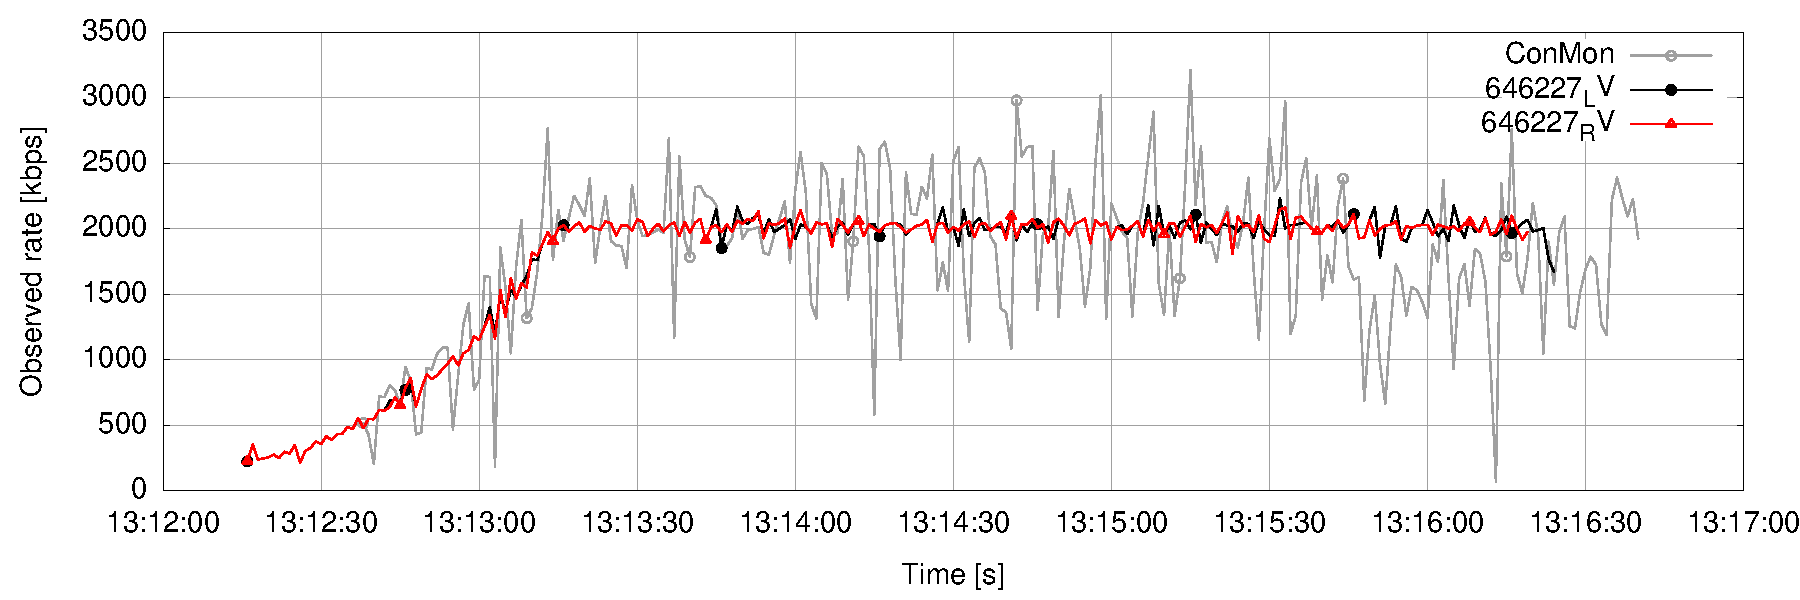
\includegraphics[width=1\textwidth]{./figures/onetoone_wifi_statsconmon.pdf}
      \caption[Point-to-point video stream plot using StatsAPI and ConMon data over WiFi]{Point-to-point video stream plot using StatsAPI and ConMon data over WiFi.}
	\label{fig:onetooneWifistatsconmon}
\end{figure}

Figure~\ref{fig:onetooneWifistatsconmon} represents the throughput rate on the same video stream, the three lines are the comparison between local video stream in origin peer, remote video stream in receiver peer and {\it ConMon} capture of the remote video stream on the receiver peer. All three streams contain the same data but they are measured in different layers, this will help us to understand the difference of throughput that is handling the overhead of the RTP and the disruption caused by the WiFi network.

Notice that red and black colors represent the Local Video (LV) and Remote Video (RV) from the same SSRC, both captures indicate the same stream captured using {\it StatsAPI}, and the grey line plots the capture performed using {\it ConMon} of the same SSRC. It is easy to observe that both {\it StatsAPI} captures are similar, some offset is produced due to the processing time between the network layer and the browser API that returns all values. Besides this, the capture is neat and throughput at the output of the origin client and input of the receiver is similar. Capture in the network layer is more abrupt as all packets are captured and the period of calculus when plotting affects when the value is added, when having two opposite values peaks they should be balanced, meaning that the transmission in most of the period is stable and the peaks when plotting are a result of accuracy. Call duration in this test has been around five minutes. Some areas, mostly between 13.15.30 and 13.16.00, show a strange behavior of the link that might be produced by the WiFi, this throughput distortion is balanced on the WebRTC layer as the throughput delivered by the API does not change.

When we try to measure the quality of the call one important indicator is the delay, to calculate the delay we can either use the RTT measured by our {\it StatsAPI} or use the captures performed on the network layer by {\it ConMon}. The {\it ConMon} procedure will give us a high accuracy on the delay subtracting both timestamps from both of the clients, this will require to reduce the drift of the internal clock of the computers.

 \begin{figure}[h]
  \centering
    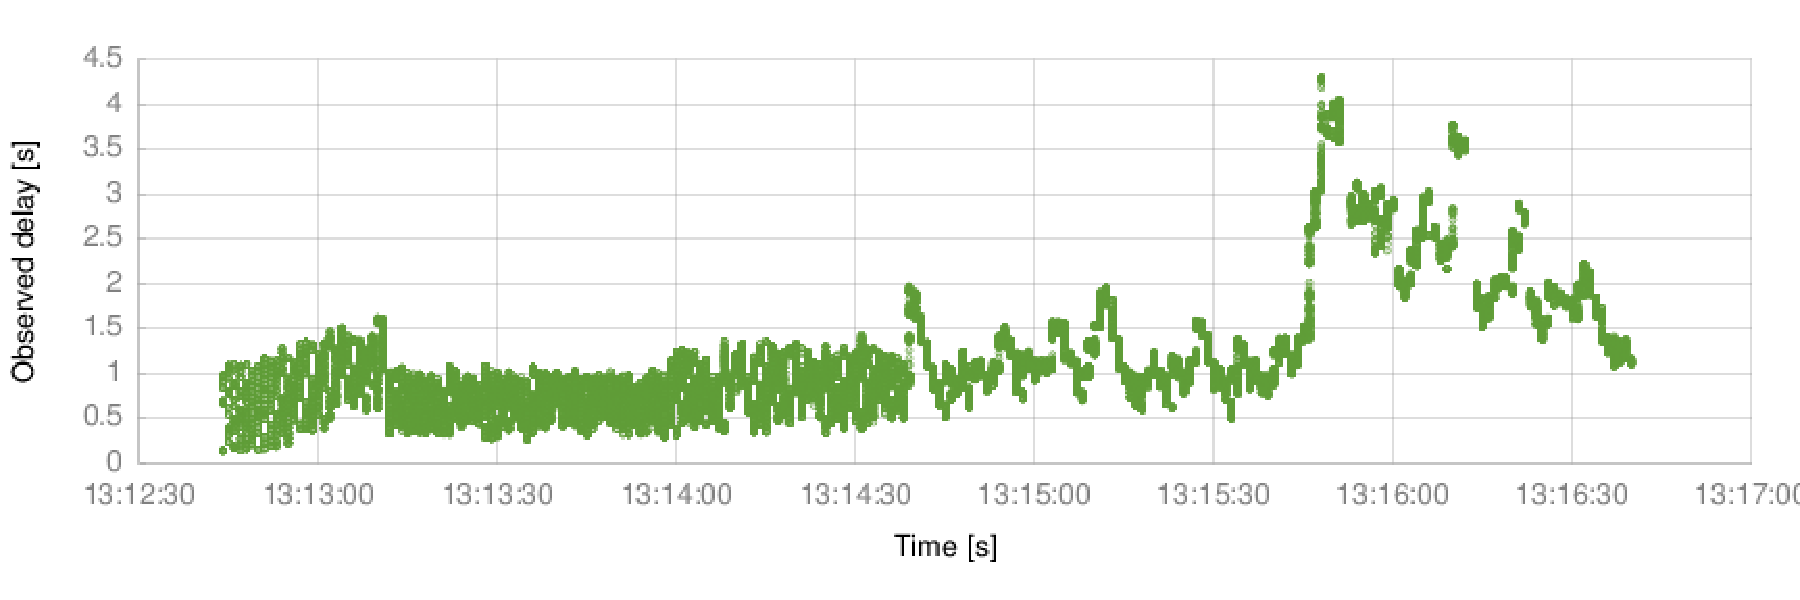
\includegraphics[width=1\textwidth]{./figures/delay_116_646227.pdf}
      \caption[Delay calculated on the same stream captured using ConMon in both ends over WiFi]{Delay calculated on the same stream captured using ConMon in both ends over WiFi.}
	\label{fig:delay_116_646227}
\end{figure}

Figure~\ref{fig:delay_116_646227} represents the delay of the stream plotted in~\ref{fig:onetooneWifistatsconmon}. We can see that the quality of the call is affected by the network distortion at the end of Figure~\ref{fig:onetooneWifistatsconmon}, this variation of the throughput delivers a high delay of more than 4 seconds during some period of time between 13:15:30 and 13:16:30, the media received at that time will not render correctly and the user experience of the call is going to be worst than at the beginning of the call. A bursty WiFi network will led to delay even the bandwidth seems to be stable.

\subsubsection{Non-constrained link test}

After seeing how WebRTC performs in WiFi  we are going to proceed with all tests in a controlled wired scenario adding different constraints to the link. This tests will be automated running ten iterations every time in order to get as much accurate results as possible.
 
 \begin{figure}[h]
  \centering
    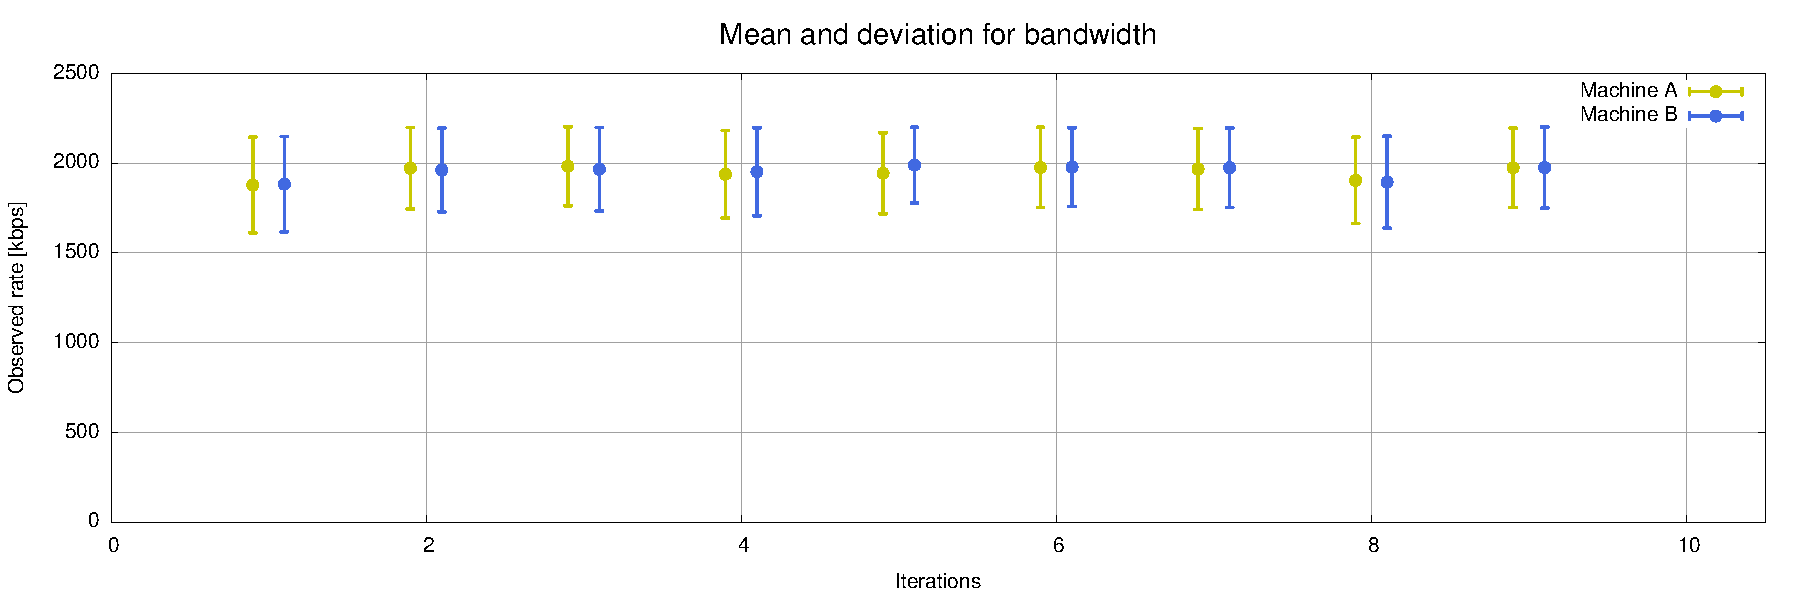
\includegraphics[width=1\textwidth]{./figures/no_ipfw.pdf}
      \caption[Bandwidth results for non-conditioned link]{Bandwidth results for non-conditioned link.}
	\label{fig:no_ipfw}
\end{figure}

Figure~\ref{fig:no_ipfw} plots the average bandwidth of every call in a wired network without any link condition, the average bandwidth obtained in the test is 1949.7 Kbit/s with 233 Kbit/s of deviation which gives the conclusion of having approximately 2 Mbit/s standard bandwidth in a video stream for a non-conditioned link in WebRTC. Delay result in 5.1 ms with 1.5 ms deviation and RTT about 9.5 ms. Those results can be taken as standard for a non-conditioned WebRTC with high bandwidth resources. A summary of results is shown in Table~\ref{fig:p2p_no_ipfw}. Some interesting results to track is the amount of calls failed in every test, considering all those calls go through a TURN server we might be able to approximate the success rate when establishing calls. All results go along with the deviation being this an important factor, in this test without any link conditioner we might have small deviation values such as milliseconds, but when adding conditions to the link those values will grow carrying less accuracy.
Setup time is stablished as the time it take since the start of the PeerConnection object until the media stream from the other peer arrives, this value directly affects the time it takes for a user to be able to start talking, in the optimal environment it takes about 1.5 seconds to start the call. We also had zero packet losses and two calls that failed to succeed using TURN in the standard environment.

\begin{table}
\begin{center}
    \begin{tabular}{c D{,}{\pm}{-1} D{,}{\pm}{-1} D{,}{\pm}{-1} }
   	 \toprule
	\textit{}
	& \multicolumn{1}{c}{\textit{Machine A}}
	& \multicolumn{1}{c}{\textit{Machine B}}
	& \multicolumn{1}{c}{\textit{Overall}}\\
	\midrule
	\textbf{CPU (\%)} & 48.76 ,2.76 & 48.83 ,2.78 & 48.79 ,2.77\\
	\textbf{Memory (\%)} & 35.98 ,0.3 & 36.43 ,0.29 & 36.21 ,0.29\\
	\textbf{Banddwidth (Kbit/s)} & 1947.61 ,232.75 & 1951.76 ,234.5 & 1949.7 ,233.62\\
	\textbf{Setup time (ms)} & 1436.33 ,25 & 1447.44 ,22.71 & 1441.88 ,24.04\\
	\textbf{RTT (ms)} & 9.49 ,2.11 & 9.64 ,2.71 & 9.57 ,2.41\\
	\textbf{Delay (ms)} & 4.84 ,1.5 & 5.4 ,1.53 & 5.12 ,1.52\\
	\bottomrule
    \end{tabular}
    \caption[P2P test with no link conditions]{P2P test with no link conditions.}
    \label{fig:p2p_no_ipfw}
\end{center}
\end{table}

Delay values in Table~\ref{fig:p2p_no_ipfw} are represented as a mean calculation of all the delay obtained in the link, thus this value is not representative of what happened in the call. Considering the example in Figure~\ref{fig:delay_116_646227} we can see that the delay can variate during the call being the mean not appropriate to measure the response against the conditions of the link. In order to observe the behavior of WebRTC in delay we have two different approaches, the mean delay with deviation and delay distribution of all calls. 

 \begin{figure}[h]
  \centering
    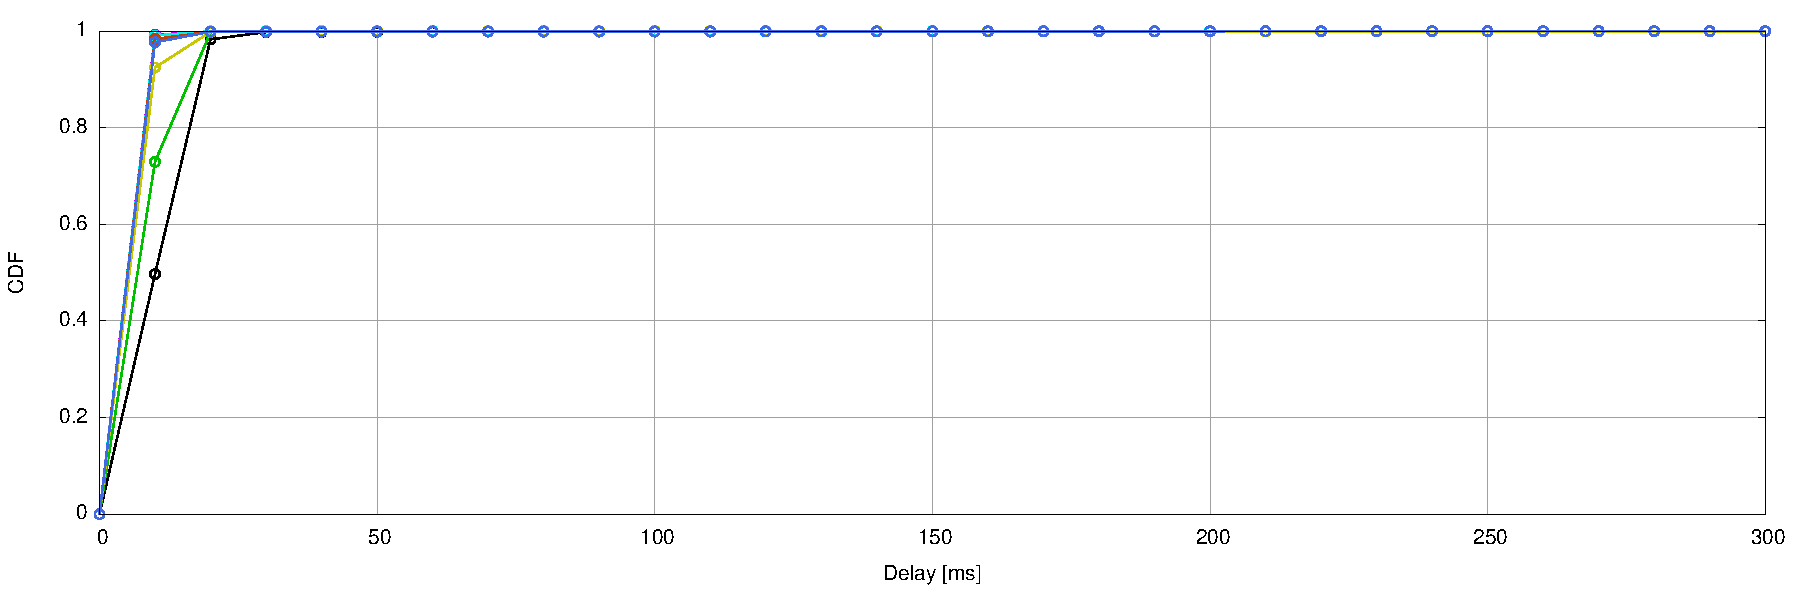
\includegraphics[width=1\textwidth]{./figures/total_delay_distribution_no_ipfw.pdf}
      \caption[Delay distribution in each P2P iterations with no link constraints]{Delay distribution in each P2P iterations with no link constraints.}
	\label{fig:total_delay_distribution_no_ipfw}
\end{figure}

 \begin{figure}[h]
  \centering
    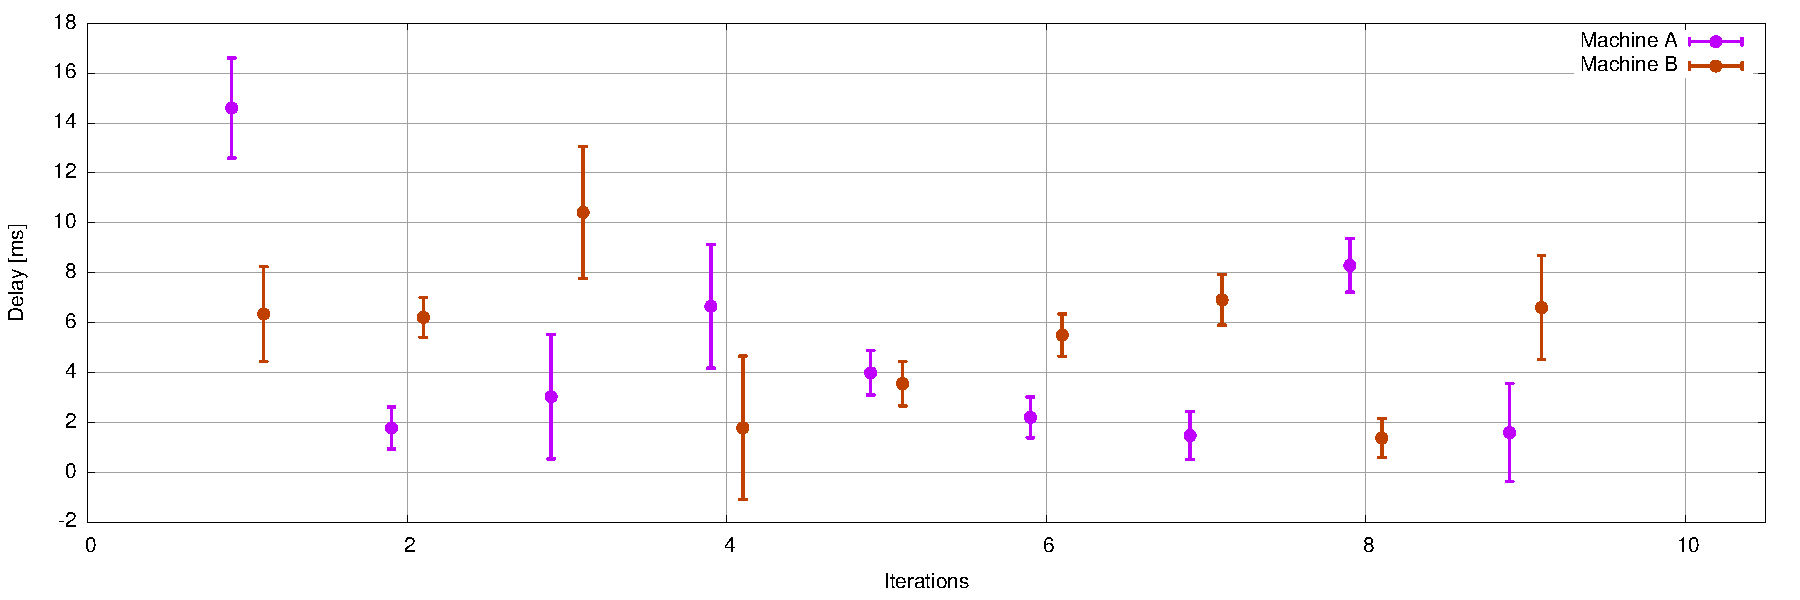
\includegraphics[width=1\textwidth]{./figures/mean_deviation_delay_no_ipfw.pdf}
      \caption[Mean and deviation for delay in each P2P iterations with no link constraints]{Mean and deviation for delay in each P2P iterations with no link constraints.}
	\label{fig:mean_deviation_delay_no_ipfw}
\end{figure}

Figure~\ref{fig:mean_deviation_delay_no_ipfw} represents the mean and deviation of delay calculated for all iterations, this delay is calculated on basis with the arrival timestamp for each packet with the captures performed in both sides by {\it ConMon}. We run an NTPD daemon to calculate the drift on the time and sync both machines.  There is small amount of drift of maximum 3ms in the worst case and as small as 1ms in the best one. In Figure~\ref{fig:total_delay_distribution_no_ipfw}, the distribution is given by the amount of packets that have some specific amount of delay, they are counted by batches of 10ms with a maximum range of 300ms. Most of the packets run with less than 25ms delay in all the iterations. The user experience with this small amount of delay with no aggressive steps in the plot will be barely negligible. Figures~\ref{fig:mean_deviation_delay_no_ipfw} and~\ref{fig:total_delay_distribution_no_ipfw} differentiate from Figure~\ref{fig:delay_116_646227} in the measurement of a global delay for an specific constraint scenario instead of just plotting a single call case, many aspects may affect the delay and the an optimal way to observe it is to plot the distribution and deviation of each iteration and try to guess a patron that repeats, Figure~\ref{fig:delay_116_646227} is good to observe just one call if we add some conditions to the link meanwhile the call is going on.

\subsubsection{Behavior in lossy environments}

We have performed some tests regarding lossy environments to see how WebRTC behaves in those, lossy situations can be given with some mobile environments with low coverage or just by having a busy link with no resources available.

We have tested the topology with 1, 5, 10 and 20\% of packet loss, according to the results in Table~\ref{fig:p2p_packet_bw} we are seeing a pretty good response from the internal algorithm up to 5\% with small effect to the bandwidth and delay. When running with 10\% loss the bandwidth drops to an average of 1140.8 Kbit/s and 162 Kbit/s deviation which is half of the corresponding amount for an standard call, this affects the quality of the link and video, 20\% loss will affect to the performance dropping the bandwidth to an average of 314.4 Kbit/s with 62 Kbit/s deviation. We can say that the video quality will be worst with lossy networks but the delay is not affected, having a delay distribution response that matches the standard case without affecting the way users will talk, quality will be worst but the call will be correct in terms of usage. All metrics are in the normal range except bandwidth.

The algorithm used in WebRTC regarding to packet loss is proven to work fine in lossy environments with the results obtained, but there is a big gap of performance in the 10\% loss network compared to the results with 20\%, it is obviously a big amount of packets but the response with 20\% is significantly better than the one with 10\%.

\begin{table}
\begin{center}
    \begin{tabular}{c D{,}{\pm}{-1} D{,}{\pm}{-1} D{,}{\pm}{-1} }
   	 \toprule
	\textit{}
	& \multicolumn{1}{c}{\textit{Machine A}}
	& \multicolumn{1}{c}{\textit{Machine B}}
	& \multicolumn{1}{c}{\textit{Overall}}\\
	\midrule
	\textbf{1\% (Kbit/s)} & 1913.59 ,252.11 & 1880.24 ,261.46 & 1896.91 ,256.78\\
	\textbf{5\% (Kbit/s)} & 1609.65 ,158.46 & 1527.84 ,198.59 & 1568.74  ,178.52\\
	\textbf{10\% (Kbit/s)} & 1166.70 ,145.96 & 1114.94 ,177.88 & 1140.82 ,161.92\\
	\textbf{20\% (Kbit/s)} & 333.34 ,65.99 & 295.46 ,57.98 & 314.4 ,61.98\\
	\bottomrule
    \end{tabular}
    \caption[Averaged bandwidth with different packet loss conditions]{Averaged bandwidth with different packet loss conditions.}
    \label{fig:p2p_packet_bw}
\end{center}
\end{table}

The amount of packets lost in every test is slightly lower than the exact percentage of loss because the use of Forward Error Correction in WebRTC in Chrome, this mechanism is used to control errors in data connection with noisy channels that led to packet losses. FEC is not a must feature to implement in WebRTC but Chrome carries it as default.

When using FEC the sender encodes the message in a redundant way, by having this redundancy the receiver is able to detect a limited number of errors and autocorrect those errors without requiring retransmission.

\subsubsection{Delayed networks}

Another interesting situation that are given in mobile environments and queued networks is delay, we have also tested the performance of WebRTC in those conditions. We have benchmarked tests in different one-way delays, 50, 100, 200 and 500ms. In our case, the RTT results should be multiplied by two.

We have noticed that the system performs badly when having even small delays up to 100ms. The response of WebRTC is to reduce the bandwidth by discarding packets, this means that the congestion control systems that act in those environments are not working correctly. On the other hand, delay output does behave correctly having a continuous delay of the according time configured in the constraints, there are no sudden increases of delay and the deviation in delay fits in the standard limits.

Table~\ref{fig:p2p_delay_bw} represents the bandwidth response to the delay conditions, it is interesting to see that the deviation with the biggest delay is smaller than expected. Only with 50ms the system will output a good quality call, when increasing delay the performance of the video will decrease. WebRTC uses VP8 codec which degrades gracefully the quality in packet loss and delay conditions but the response in this case should be better if the congestion mechanisms worked properly.

\begin{table}
\begin{center}
    \begin{tabular}{c D{,}{\pm}{-1} D{,}{\pm}{-1} D{,}{\pm}{-1} }
   	 \toprule
	\textit{}
	& \multicolumn{1}{c}{\textit{Machine A}}
	& \multicolumn{1}{c}{\textit{Machine B}}
	& \multicolumn{1}{c}{\textit{Overall}}\\
	\midrule
	\textbf{50ms (Kbit/s)} & 1909.31 ,258.09 & 1917.81 ,251.62 & 1913.56 ,254.86\\
	\textbf{100ms (Kbit/s)} & 1516.07 ,263.43 & 1453.94 ,272.79 & 1485 ,268.11\\
	\textbf{200ms (Kbit/s)} & 503.71 ,116.45 & 617.92 ,142.69 & 560.82 ,129.57\\
	\textbf{500ms (Kbit/s)} & 303.58 ,59.22 & 207.77 ,32.48 & 255.67 ,45.85\\
	\bottomrule
    \end{tabular}
    \caption[Summary of averaged bandwidth with different delay conditions]{Summary of averaged bandwidth with different delay conditions.}
    \label{fig:p2p_delay_bw}
\end{center}
\end{table}

We can also observe that every iteration follows a different pattern even having an averaged result, Figure~\ref{fig:mean_deviation_bw_delay200} show the test performed at 200ms and the iterations that fail to keep a constant rate making the amount of artifacts in the video affect the quality of the call. We can certainly confirm that the methods that WebRTC should use to control the congestion in the call are not working as they should.

The problem with WebRTC relies in the usage of RTP over UDP for packet transport as UDP does not carry congestion control mechanisms that TCP does, when having real time media adapting the encoding to accommodate the varying bandwidth is difficult and cannot be done rapidly.

 \begin{figure}[h]
  \centering
    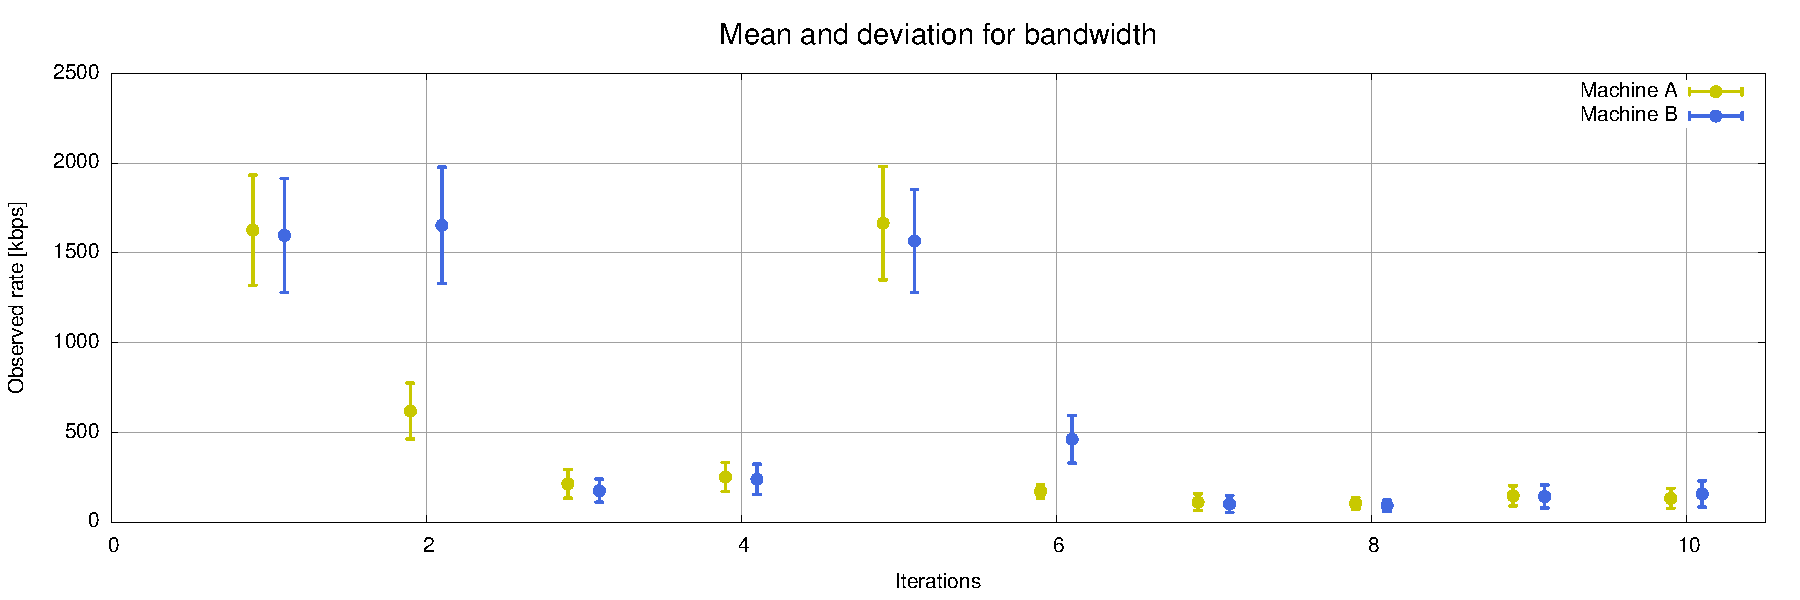
\includegraphics[width=1\textwidth]{./figures/mean_deviation_bw_delay200.pdf}
      \caption[Mean and deviation for P2P 200 ms delay test]{Mean and deviation for P2P 200 ms delay test.}
	\label{fig:mean_deviation_bw_delay200}
\end{figure}

Low latency networks will play a big role when WebRTC extends to mobile devices and the ability to react properly to delays and packet losses will be crucial for the success of WebRTC in those environments against its competitors.

\subsubsection{Bandwidth and queue variations}

We have also performed a different set of tests modifying the bandwidth and queue length. For this part of the test we have chosen to run 500 Kbit/s, 1, 5 and 10 Mbit/s with different queue sizes ranging from 100 ms, 500 ms, 1s and 10 s. In total we have run 12 different tests with ten iterations each.

The queue size is set in slots to {\it Dummynet} considering each slot as standard ethernet packet of 1500 Bytes, to calculate this number we use Equation~\ref{eq:QueueSize}.

\begin{equation}
	\frac{Bandwidth (Bits)}{8 \times 1500} \times Queue (seconds)
	\label{eq:QueueSize}
\end{equation}

We have seen a good response when having big queue size but larger deviation in bandwidth when reducing this queue size to 100 ms or 500 ms, this produced high delays over 20 ms for every call with different distribution curves. The delay that is given to the duration of the call is not stable and will affect the media flow, this increasing curve of delay distribution is given by the small queue size which produces bursty packets to arrive to the peer having different delay conditions.
When we tested the 5 Mbit/s case we got a strange high delay output even the bandwidth adapted to the requirements of WebRTC. The delay deviation is also high and will affect the time the packets arrive with large jittering.